\subsection{Platform-as-a-Service (PaaS)}

PaaS clouds, which have been experiencing a rapid growth in 
popularity~\cite{paas-growth,paas-growth2},
typically host web-accessible (HTTP/S) applications, to which they provide
high levels of scalability, availability, and sandboxed execution. PaaS
clouds provide scalability by automatically allocating resources for
applications on the fly (auto scaling), and provide availability through the
execution of multiple instances of the application. Applications deployed on
a PaaS cloud depend on a number of scalable services intrinsic to the 
cloud platform. Our goal is to design Roots as another intrinsic service of the PaaS cloud
so that it can function automatically and non-intrusively as an APM.
%PaaS clouds provide a high level of
%abstraction to the application developer that effectively hides all the
%infra\-structure-level details such as physical resource allocation (CPU,
%memory, disk etc), operating system, and network configuration. This enables
%application developers to focus solely on the programming aspects of their
%applications, without having to be concerned about deployment issues.
%Consequently, viable PaaS technologies as well as PaaS-hosted applications
%have been increasing rapidly in number~\cite{paas-growth,paas-growth2}.  
%But
%due to the high level of abstraction, performance monitoring and root cause
%analysis is particularly challenging in PaaS clouds. Due to this reason, and
%the large number of PaaS applications available for testing, we design Roots
%APM to operate within PaaS clouds.

\begin{figure}
\centering
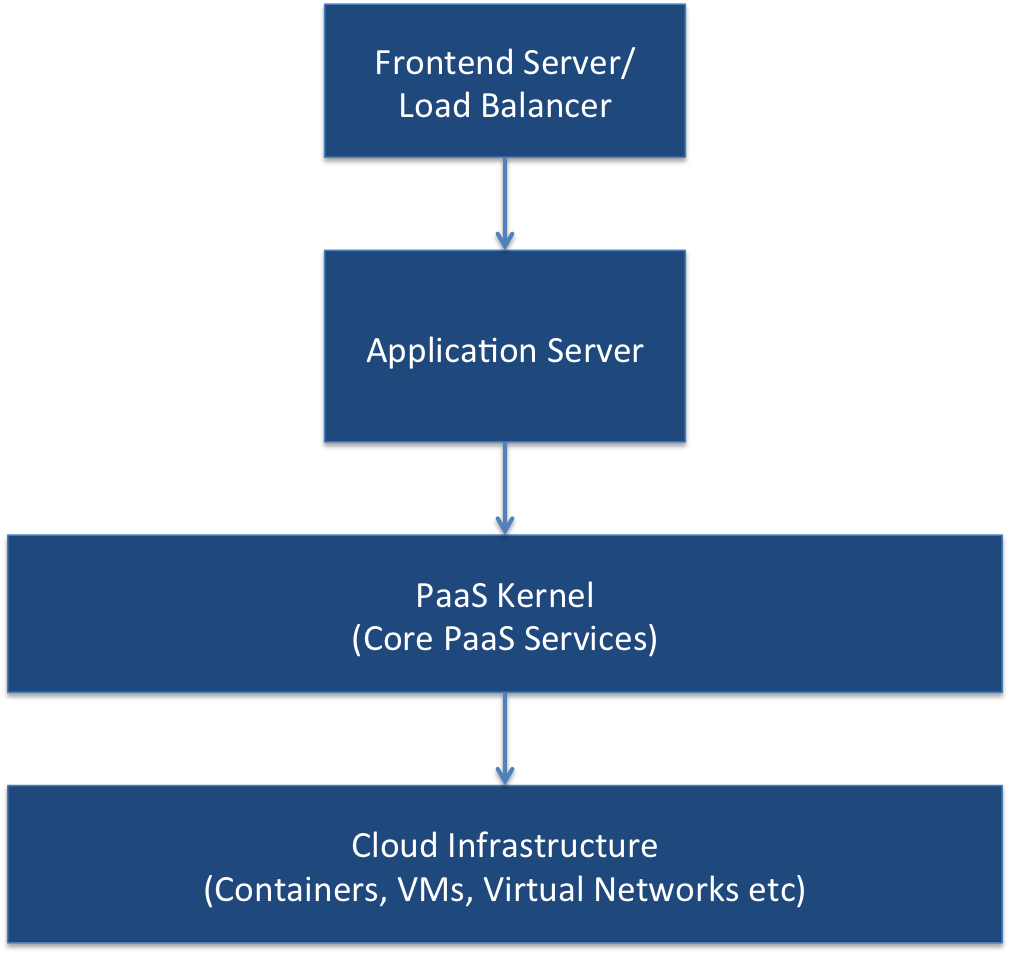
\includegraphics[scale=0.5]{paas_architecture}
\caption{PaaS system organization.}
\label{fig:paas_architecture}
\end{figure}

Figure~\ref{fig:paas_architecture} shows the key layers of a typical PaaS cloud. Arrows indicate
the flow of data and control in response to application requests.
At the lowest level of a PaaS cloud is an infrastructure that consists of the necessary compute, storage
and networking resources. How this infrastructure is set up may vary from a simple cluster of physical 
machines to a comprehensive Infrastructure-as-a-Service (IaaS) cloud. In large scale PaaS clouds,
this layer typically consists of many virtual machines and/or containers with the ability to acquire more
resources on the fly.

On top of the infrastructure layer lies the PaaS kernel. This is a collection of managed, scalable
services that high-level application developers can compose into their applications. The provided services
may include database services, caching services, queuing services and much more. Some PaaS clouds
provide a managed set of APIs (a ``software development
kit'' or SDK) for the application developer to access these fundamental services. 
In that case all interactions between the applications and the PaaS kernel must take place through
the cloud provider specified APIs (e.g. Google App Engine~\cite{gae}). 

One level above the PaaS kernel we find the application servers that are used to deploy and run
applications. Application servers provide the necessary integration (linkage) between application code and the
underlying PaaS kernel, while sandboxing application code for secure, multi-tenant operation. On top
of the application servers layer resides the request
front-end and load balancing layer. This layer is responsible
for receiving all application requests, filtering them and routing them to an appropriate application
server instance for further execution. Front-end server is therefore the entry point for PaaS-deployed
applications for all application clients.

Each of the above layers can span multiple processes, running over multiple physical or virtual
machines. Therefore the execution of a single application request typically involves cooperation
of multiple distributed processes and/or machines. In order to perform comprehensive monitoring
and root cause analysis, we need to be able to monitor each of the above layers along with their
enclosed components. Further, we need to be able to trace the flow of data and control
across different layers and components.

\subsection{Cloud-hosted Web Applications} 

%\textcolor{blue}{You might want to move some of this discussion into the
%introduction since it allows the reader to understand the focus of the work we
%present.}
%Added more details about PaaS services to the intro

Our work concentrates on the web
applications deployed in PaaS clouds. An application of this nature exposes
one or more web application programming interfaces (web APIs) through which
clients can interact with it. The web APIs accept HTTP/S requests sent by
remote clients, and respond with machine readable responses (e.g. HTML, JSON,
XML, Protocol Buffers~\cite{protobuff}). This type of applications tend to be highly
interactive, and clients typically have strict expectations on the application
response time. Studies have shown that poor application response
time may even lead to revenue loss~\cite{latency-matters}.
Additionally, the PaaS cloud on
which an application is running may impose additional constraints on the
application response time for scalability
reasons~\cite{azure-limits,gae-limits}.  For example Google App Engine
requires that no application request takes more than 60 seconds to execute.

PaaS-hosted web applications rely on various PaaS kernel services offered by the underlying
cloud platform. By offloading common application functionality such as data storage, caching,
user management, and security to a set of managed cloud services, application developers
can greatly reduce the amount of code they have to write. It also eliminates the need to install, run and
manage many other support software that would otherwise be necessary (e.g. a database server, 
a message broker etc.). In other words, when developing applications for a PaaS environment, the
developer just focuses on implementing his/her application code
using the available PaaS services. All deployment and utility services are provisioned 
by the PaaS cloud itself. 

The downside of this approach is that application developers no longer have full runtime visibility
into the application execution. Since most of the application functionality is provided by a set 
of PaaS kernel services that are in cloud provider's domain, the application
developer does not have total control over application performance. If the application 
response time becomes too slow, the application developer is not in a position to determine
where in the entire cloud platform the performance bottleneck is due to the opacity of the cloud
platform's internal implementation. 

One way to circumvent this 
limitation is to instrument application code, and continuously monitor the time taken by various
parts of the application. But this activity can be tedious for the application developer, 
may be error prone thereby misleading those attempting to
diagnose a problem, and
the additional code instrumentation may slow down or alter the application's
performance. 
%Also there is no way to enforce correct, and consistent instrumentation of application code.  
%That is, the application developers must be careful in gathering and storing the appropriate
%runtime data. Otherwise their analyses will be inaccurate.
Implementing data collection and analysis as a service built into the PaaS cloud allows 
anomaly detection and bottleneck identification to be a ``curated'' service that is 
reliably managed by the cloud platform.

\subsection{Performance Anomalies}
In this work we define \textit{anomalies} as application performance change events that cause
one or more performance SLOs to be violated. Our model is
one in which the clients of a web application have engaged in a
``service-level agreement'' (SLA)
with the ``owner'' or operator of the application that is hosted in a PaaS.  The SLA
stipulates a response-time ``service-level objective'' (SLO) that, if violated, constitutes a breech of the
agreement.
%approach associates each application with
%a set of performance SLOs. We consider SLOs concerning the application response time
%(latency), which get violated when an application becomes too slow.
If the performance of an application deteriorates to the
point that at least one of its SLOs is violated, we treat it as an anomaly. Moreover, the process
of diagnosing the reason for 
an anomaly is referred to as \textit{root cause analysis}.
For a given anomaly, the root cause could be a change in the application workload or
a \textit{bottleneck} in the application runtime. Bottlenecks may occur in the application code, 
or in the PaaS services that the application rely on.

In order to maintain a satisfactory level of user experience and adhere to any previously
agreed upon performance SLOs, application developers and cloud administrators wish
to detect performance anomalies as soon as they occur. When detected, they
must perform root cause analysis to identify the cause of the anomaly, and take some
corrective and/or preventive action. 
This diagnosis usually occurs as a two step process. First, one must determine
whether the anomaly was caused by a change in the workload (e.g. a sudden 
increase in the number of client requests). If that is the case,
the resolution typically involves allocating more resources to the application or spawning
more instances of the application for load balancing purposes. If the anomaly cannot be 
attributed to a workload change, one must go another step to find the bottleneck component
that has given rise to the issue at hand.

%Detecting performance anomalies
%requires continuous monitoring of application performance which could be tedious with
%cloud platforms in use today. It is even more challenging to perform root cause analysis
%due to the complexity and the blackbox nature of the cloud platforms. 

Note that there are several
third party cloud monitoring solutions available today which provide some performance
anomaly detection support~\cite{newrelic,datadog,dynatrace}. 
However, they require additional configuration, are expensive
and cannot support root cause analysis across the entire cloud stack since they do not
have visibility into all components of the cloud
platform.